\documentclass{beamer}
\usepackage[T1]{fontenc}
\usepackage[english]{babel}
\usepackage{lmodern}
\usepackage{amsmath,amssymb}
\usepackage{algorithm}
\usepackage{algorithmic}
\usepackage{graphicx}
\usepackage{subcaption}
\usepackage{caption}
\usepackage{tikz}
\usetikzlibrary{overlay-beamer-styles}
\usepackage{booktabs,multicol,stackengine}
\usepackage[table,dvipsnames]{xcolor}
\usepackage{cancel}
\usepackage{moresize}
\usepackage{hyperref}

\usepackage{listings}
\definecolor{nus-orange}{RGB}{239,124,0}
\definecolor{nus-blue}{RGB}{0,61,124}
\definecolor{halfgray}{gray}{0.55}

\lstset{
  basicstyle=\ttfamily\footnotesize,
  keywordstyle=\bfseries\color{nus-blue},
  stringstyle=\color{ForestGreen},
  numbers=left,
  numberstyle=\scriptsize\color{halfgray},
  rulesepcolor=\color{nus-orange},
  frame=shadowbox,
  columns=flexible,
  showstringspaces=false,
  keepspaces=true,
  tabsize=2,
  breaklines=true
}

\renewcommand{\figurename}{Figure}
\renewcommand{\algorithmname}{Algorithm}

\usepackage{SHU}
\input{macros}

\title{BT5110: Tutorial 1 — Relational Model}
\author{\href{https://pratik2358.github.io/}{Pratik Karmakar}}
\institute{School of Computing,\\ National University of Singapore}
\date{AY26/27 S1}

\begin{document}

\begin{frame}
  \titlepage
  \IfFileExists{nus-logo.png}{
    \begin{figure}[htpb]\centering
      
\includegraphics[keepaspectratio, scale=0.18]{nus-logo.png}
    \end{figure}
  }{}
\end{frame}

\section{Relational Model Basics}

\begin{frame}{What is the relational model? (in plain words)}
\begin{itemize}
  \item Think \textbf{spreadsheets}: each \textbf{table} is a sheet, \textbf{rows} are items, \textbf{columns} are properties.
  \item Formally, a table is a \textbf{relation}; a row is a \textbf{tuple}; a column is an \textbf{attribute}.
  \item Each table has a rule for what counts as a valid row: that rulebook is the \textbf{schema}.
  \item Tables can be \textbf{linked}—a value in one table points to a matching value in another.
  \item Why it’s powerful: simple structure, \textbf{strong guarantees} (constraints, transactions), and \textbf{declarative} querying (SQL).
\end{itemize}
\end{frame}

\begin{frame}{Everyday analogy}
\begin{columns}[T,onlytextwidth]
\begin{column}{0.55\linewidth}
\textbf{Students} table
\begin{itemize}
  \item One row per student
  \item Columns: \texttt{email}, \texttt{name}, \texttt{faculty}, \texttt{department}, \texttt{join}
  \item \textbf{Primary key} (\texttt{email}) uniquely identifies a student
\end{itemize}
\medskip
\textbf{Books} table
\begin{itemize}
  \item One row per book title
  \item Columns: \texttt{isbn13} (PK), \texttt{isbn10}, \texttt{title}, \texttt{authors}, \texttt{publisher}, \texttt{year}
\end{itemize}
\end{column}
\begin{column}{0.45\linewidth}
\textbf{Copies \& Loans}
\begin{itemize}
  \item \texttt{copy(owner, book, copy, ...)}
  \item \texttt{loan(owner, book, copy, borrowed, returned)}
  \item \textbf{Foreign keys} connect:
  \begin{itemize}
    \item \texttt{copy.owner} $\to$ \texttt{student.email}
    \item \texttt{copy.book} $\to$ \texttt{book.isbn13}
    \item \texttt{loan.(owner, book, copy)} $\to$ \texttt{copy}
  \end{itemize}
\end{itemize}
\end{column}
\end{columns}
\end{frame}

\begin{frame}{Keys, relationships, and constraints}
\begin{itemize}
  \item \textbf{Primary key (PK)}: a column (or set) that uniquely identifies each row.
  \item \textbf{Foreign key (FK)}: a column whose values must match a PK in another table.
  \item \textbf{Domain \& CHECK constraints}: control valid values (e.g., dates, non-negative pages).
  \item \textbf{Entity integrity}: PK cannot be \texttt{NULL}.
  \item \textbf{Referential integrity}: FK must reference an existing PK (or be \texttt{NULL} if allowed).
  \item These rules keep data \textbf{consistent} across tables.
\end{itemize}
\end{frame}

\begin{frame}{How we ask questions (SQL mirrors simple ops)}
\begin{columns}[T,onlytextwidth]
\begin{column}{0.55\linewidth}
\textbf{Core ideas}
\begin{itemize}
  \item \textbf{Filter} rows (\emph{selection, $\sigma$}): \texttt{WHERE}
  \item \textbf{Pick} columns (\emph{projection, $\pi$}): \texttt{SELECT} list
  \item \textbf{Match} tables (\emph{join, $\bowtie$}): \texttt{JOIN ... ON}
  \item \textbf{Summarize} (\emph{group/aggregate}): \texttt{GROUP BY}, \texttt{COUNT}, \texttt{SUM}, \dots
\end{itemize}
\end{column}
\begin{column}{0.45\linewidth}
\textbf{Example questions}
\begin{itemize}
  \item “Which copies are currently on loan?”
  \item “Which students own at least two books?”
  \item “How many Chemistry students borrowed in 2024?”
\end{itemize}
\end{column}
\end{columns}
\vspace{0.6em}
\textbf{Takeaway:} you describe \emph{what} you want; the database figures out \emph{how} to get it efficiently (query optimization).
\end{frame}

\section{Relational Algebra Basics}

\begin{frame}{Why Relational Algebra?}
\begin{itemize}
  \item \textbf{Foundation of SQL}: Relational algebra provides the formal, mathematical basis for relational databases.
  \item Defines \textbf{operations on relations} that always produce relations.
  \item Ensures queries are \textbf{precise}, \textbf{composable}, and \textbf{optimizable}.
  \item SQL = (mostly) declarative syntax built on these algebraic ideas.
\end{itemize}
\end{frame}

\begin{frame}[fragile]{Core Operators}
\begin{itemize}
  \item \textbf{Selection ($\sigma$)}: Pick rows that satisfy a condition.  
  \(\;\;\sigma_{\text{year}=2024}(\text{Student})\)
  \item \textbf{Projection ($\pi$)}: Pick certain columns.  
  \(\;\;\pi_{\text{name, email}}(\text{Student})\)
  \item \textbf{Renaming ($\rho$)}: Rename relation/attributes.  
  \(\;\;\rho_{S}(\text{Student})\)
  \item \textbf{Union ($\cup$)}, \textbf{Difference ($-$)}, \textbf{Intersection ($\cap$)}: Set-like ops (schemas must match).
  \item \textbf{Cartesian Product ($\times$)}: Pair all tuples across two relations.
  \item \textbf{Join ($\bowtie$)}: Combine rows across relations on matching attributes.
\end{itemize}
\end{frame}

\begin{frame}[fragile]{Examples and SQL Mapping}
\begin{columns}[T,onlytextwidth]
\begin{column}{0.55\linewidth}
\small
\textbf{Relational Algebra}
\begin{itemize}
  \item $\pi_{\text{name}}(\sigma_{\text{faculty}=\text{'SoC'}}(\text{Student}))$
  \vspace{1.1cm}
  \item $\text{Student} \bowtie_{\text{student.email}=\text{copy.owner}} \text{Copy}$
  \vspace{1.1cm}
  \item $\pi_{\text{isbn13}}(\text{Book}) - \pi_{\text{book}}(\text{Copy})$
\end{itemize}
\end{column}
\begin{column}{0.45\linewidth}
\textbf{SQL Equivalent}
\begin{lstlisting}[language=SQL]
SELECT name
FROM student
WHERE faculty = 'SoC';
\end{lstlisting}
\begin{lstlisting}[language=SQL]
SELECT *
FROM student s
JOIN copy c
  ON s.email = c.owner;
\end{lstlisting}
\begin{lstlisting}[language=SQL]
SELECT isbn13
FROM book
EXCEPT
SELECT book
FROM copy;
\end{lstlisting}
\end{column}
\end{columns}
\end{frame}

\begin{frame}{Takeaway}
\begin{itemize}
  \item Relational algebra = the \textbf{mathematical core} of querying.
  \item SQL extends it with ordering, grouping, aggregation, etc.
  \item Understanding algebra clarifies how SQL queries work “under the hood.”
\end{itemize}
\end{frame}

\section{Question}

\begin{frame}{Case Description}
\small
Students at the National University of Ngendipura (NUN) buy, lend, and borrow books.
Your company, Apasaja Private Limited, is commissioned by NUN Students Association (NUNStA) to implement an online book exchange system that records information about students and the books they own, borrow, and lend.

The database stores:
\begin{itemize}
  \item \textbf{Students}: name, faculty, department, \texttt{join} date, graduation date. Identifier: \texttt{email}.
  \item \textbf{Books}: title, format, pages, language, authors, publisher, publication date, \texttt{ISBN-10}, \texttt{ISBN-13}.
  \item \textbf{Loans}: per-copy borrow and return dates.
\end{itemize}
A book may exist with no current owner (owner graduated, or a lecturer recommended it before any student bought it).
Auditing: books, copies, and students are retained while referenced by an existing copy or loan record.
\end{frame}

\begin{frame}{Q1. Data Definition Language (DDL)}
\textbf{(a)} Download from \texttt{Canvas $\triangleright$ Files $\triangleright$ Cases $\triangleright$ Book Exchange}:\\
\texttt{NUNStASchema.sql}, \texttt{NUNStAClean.sql}, \texttt{NUNStAStudent.sql}, \texttt{NUNStABook.sql}, \texttt{NUNStACopy.sql}, \texttt{NUNStALoan.sql}.
\vspace{0.5em}

What they do:
\begin{itemize}
  \item \textbf{Clean Up} (\texttt{NUNStAClean.sql}): drops existing tables — \texttt{DROP TABLE IF EXISTS}.
  \item \textbf{Schema} (\texttt{NUNStASchema.sql}): defines the four relations and their constraints — \texttt{CREATE TABLE}, \texttt{PRIMARY KEY}, \texttt{FOREIGN KEY}, \texttt{UNIQUE}, \texttt{NOT NULL}, \texttt{CHECK}.
  \item \textbf{Data} (\texttt{NUNStAStudent/Book/Copy/Loan.sql}): populate the tables — \texttt{INSERT INTO student}/\texttt{book}/\texttt{copy}/\texttt{loan} (order matters).
\end{itemize}
\end{frame}

\begin{frame}[fragile]{Q1. Finding and Fixing the Error}
\textbf{(b)} Running \texttt{NUNStASchema.sql} as downloaded raises an error:
\begin{lstlisting}
ERROR:  relation "copy" does not exist
\end{lstlisting}
\textbf{Cause}: the file creates tables in the order \texttt{book}, \texttt{student}, \texttt{loan}, \texttt{copy} — but \texttt{loan} declares
\begin{lstlisting}
FOREIGN KEY (owner, book, copy) REFERENCES copy(owner, book, copy)
\end{lstlisting}
so \texttt{CREATE TABLE loan} fails because \texttt{copy} does not exist yet.

\textbf{Fix}: create tables in dependency order — \texttt{book}/\texttt{student} $\to$ \texttt{copy} $\to$ \texttt{loan} — then populate \texttt{student}/\texttt{book} $\to$ \texttt{copy} $\to$ \texttt{loan}. Cleanup is the reverse.
\end{frame}

\begin{frame}[fragile]{Creating the Database}
    \begin{figure}
        \centering
        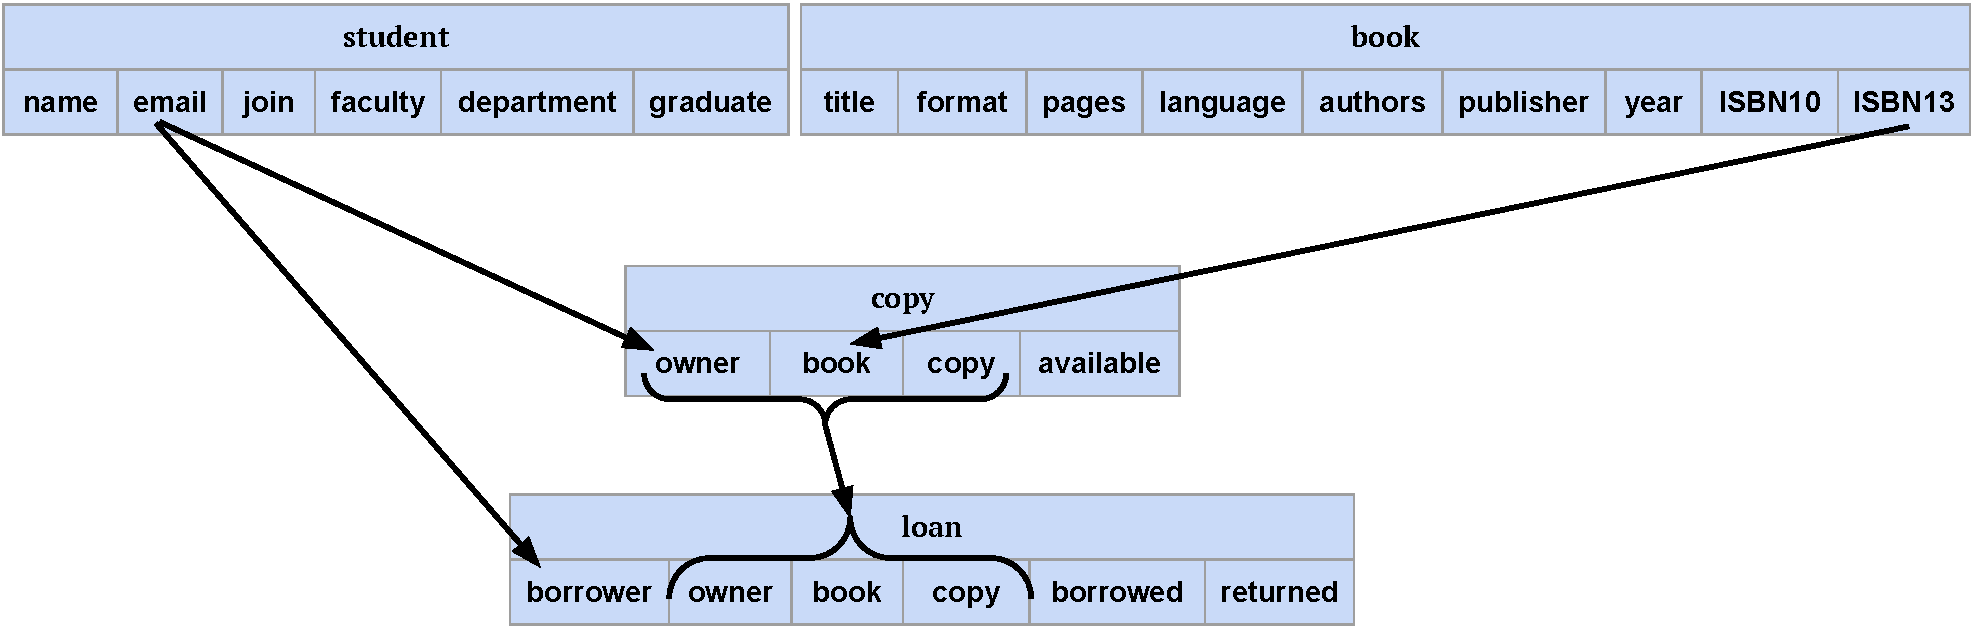
\includegraphics[width=1\linewidth]{schema_t6.pdf}
        \caption{\texttt{student} and \texttt{book} are independent tables (relations). \texttt{copy} relies on \texttt{student} for its \texttt{owner} attribute and on \texttt{book} for its \texttt{book} attribute. \texttt{loan} relies on copy for \texttt{(owner, book, copy)} attributes and on \texttt{student} for its \texttt{borrower} attribute.}
        \label{fig:depend}
    \end{figure}
\end{frame}

\begin{frame}[fragile]{Creating the Database}
    From Figure~\ref{fig:depend} it is clear that we need to populate either the \texttt{student} table or the \texttt{book} table first. Then we should populate \texttt{copy} and \texttt{loan} should be the last. \\
    \pause
    \scriptsize
    \alert{How would you find the order when the number of tables (relations) is much higher and have complex set of dependencies?} \pause \textcolor{blue}{Use Topological Sorting}\\
    \pause
    \normalsize
    In \texttt{psql} run\footnote{The order of \texttt{NUNStAStudent.sql} and \texttt{NUNStABook.sql} are interchangeable.}:
    \begin{lstlisting}
        \i NUNStAStudent.sql;
        \i NUNStABook.sql;
        \i NUNStACopy.sql;
        \i NUNStALoan.sql;
    \end{lstlisting}
Your database is now ready\footnote{You need to be in the same directory of these files for these to run. Otherwise provide the entire file paths after \texttt{\textbackslash i}.}.\\
\end{frame}

\begin{frame}{Q1. Primary Keys}
\textbf{(c)} Primary key of each relation:
\begin{itemize}
  \item \texttt{book}: \texttt{ISBN13}
  \item \texttt{student}: \texttt{email}
  \item \texttt{copy}: \texttt{(owner, book, copy)}
  \item \texttt{loan}: \texttt{(borrowed, borrower, owner, book, copy)}
\end{itemize}
\end{frame}

\begin{frame}{Q1. Foreign Keys}
\textbf{(d)} Referencing $\to$ referenced relation/attribute(s):
\begin{itemize}
  \item \texttt{copy.owner} $\to$ \texttt{student.email}
  \item \texttt{copy.book} $\to$ \texttt{book.ISBN13}
  \item \texttt{loan.borrower} $\to$ \texttt{student.email}
  \item \texttt{loan.(owner, book, copy)} $\to$ \texttt{copy.(owner, book, copy)}
\end{itemize}
\end{frame}

\begin{frame}{Q1. Composite Primary Keys}
\textbf{(e)} Which relations need more than one attribute to be uniquely identified?
\begin{itemize}
  \item \textbf{\texttt{copy} — (owner, book, copy)}: an owner can own different books, and more than one copy of the \emph{same} book; the copy number distinguishes those copies.
  \item \textbf{\texttt{loan} — (borrowed, borrower, owner, book, copy)}: uniquely identifies a loan \emph{event}, i.e.\ a particular borrower borrowing a particular physical copy on a particular date.
\end{itemize}
\end{frame}

\begin{frame}[fragile]{Q1. Constraints — UNIQUE, NOT NULL, CHECK}
\textbf{(f)} Examples and the business rule each enforces:
\begin{itemize}
  \item \textbf{UNIQUE} \texttt{book.ISBN10} — no two book records may share the same ISBN-10.
  \item \textbf{NOT NULL} \texttt{student.name, join, faculty, department} — required student information cannot be missing.
  \item \textbf{CHECK} \texttt{book.format = 'paperback' OR 'hardcover'} — only permitted book formats are stored.
  \item \textbf{CHECK} \texttt{student.graduate >= join} — a graduation date cannot be before the student joined.
  \item \textbf{CHECK} \texttt{copy.copy > 0} — copy numbers must be positive.
  \item \textbf{CHECK} \texttt{loan.returned >= borrowed} — a return date cannot be before the borrowing date.
\end{itemize}
\end{frame}

\begin{frame}[fragile]{Q2. Insert / Delete / Update — Book Inserts}
\textbf{(a)} Insert a new book:
\begin{lstlisting}[language=SQL]
INSERT INTO book VALUES (
  'An Introduction to Database Systems',
  'paperback',
  640,
  'English',
  'C. J. Date',
  'Pearson',
  '2003-01-01',
  '0321197844',
  '978-0321197849'
);
-- Verify:
SELECT * FROM book;
\end{lstlisting}
\end{frame}

\begin{frame}[fragile]{Q2. Book Variants \& Keys}
\textbf{(b)} Same book, different \texttt{ISBN13} (unique \texttt{isbn10} violated):
\begin{lstlisting}[language=SQL]
INSERT INTO book VALUES (
  'An Introduction to Database Systems',
  'paperback',
  640,
  'English',
  'C. J. Date',
  'Pearson',
  '2003-01-01',
  '0321197844',
  '978-0201385908'
);
\end{lstlisting}
\end{frame}

\begin{frame}[fragile]{Q2. Book Variants \& Keys}
\textbf{(c)} Same book, different \texttt{ISBN10} (PK \texttt{isbn13} violated):
\begin{lstlisting}[language=SQL]
INSERT INTO book VALUES (
  'An Introduction to Database Systems',
  'paperback',
  640,
  'English',
  'C. J. Date',
  'Pearson',
  '2003-01-01',
  '0201385902',
  '978-0321197849'
);
\end{lstlisting}
\end{frame}

\begin{frame}[fragile]{Q2. Insert Students}
\textbf{(d)} Insert a new student by explicitly naming the target columns. What value is stored in any omitted column?
\begin{lstlisting}[language=SQL]
INSERT INTO student (email, name, join, faculty, department) VALUES (
  'ben.lim@u.nun.edu',
  'BEN LIM',
  '2026-08-10',
  'School of Computing',
  'CS'
);
\end{lstlisting}
Insertion succeeds; the omitted \texttt{graduate} column is \texttt{NULL}.
\end{frame}

\begin{frame}[fragile]{Q2. Update \& Delete}
\textbf{(e)} Change department name from \texttt{'CS'} to \texttt{'Computer Science'}:
\begin{lstlisting}[language=SQL]
UPDATE student
SET department = 'Computer Science'
WHERE department = 'CS';
\end{lstlisting}
Every \texttt{'CS'} row is updated: 24 students originally, plus Ben Lim from (d) $\Rightarrow$ \textbf{25 rows}.

\textbf{(f)} Case-sensitive delete:
\begin{lstlisting}[language=SQL]
DELETE FROM student WHERE department = 'chemistry';
\end{lstlisting}
\textbf{0 rows} match — PostgreSQL string comparison is case-sensitive; no row stores lowercase \texttt{'chemistry'}.
\end{frame}

\begin{frame}[fragile]{Q2. Update \& Delete}
\textbf{(g)}
\begin{lstlisting}[language=SQL]
DELETE FROM student WHERE department = 'Chemistry';
\end{lstlisting}
\textbf{3 rows} match, but the \texttt{DELETE} \textbf{fails}: those students are still referenced by foreign keys in \texttt{copy} and/or \texttt{loan}, so referential integrity blocks the deletion — none of the 3 rows is removed.

\medskip
Comparing with (f): (f) matches 0 rows (case mismatch); (g) matches 3 rows but referential integrity prevents the deletion.
\end{frame}

\begin{frame}[fragile]{Q3. Modifying the Schema — Drop Redundant Availability}
\textbf{(a)} Availability is derivable: a copy is unavailable iff it has an open loan.
\begin{lstlisting}[language=SQL]
-- Unreturned loans
SELECT owner, book, copy, returned
FROM loan
WHERE returned ISNULL;

-- Remove redundant column
ALTER TABLE copy
DROP COLUMN available;
\end{lstlisting}
\end{frame}

\begin{frame}[fragile]{Q3. Modifying the Schema — Drop Redundant Availability}
\begin{lstlisting}[language=SQL]
-- View that recomputes availability
CREATE OR REPLACE VIEW copy_view (owner, book, copy, available) AS (
  SELECT DISTINCT c.owner, c.book, c.copy,
    CASE
      WHEN EXISTS (
        SELECT * FROM loan l
        WHERE l.owner = c.owner
          AND l.book  = c.book
          AND l.copy  = c.copy
          AND l.returned ISNULL
      ) THEN 'FALSE'
      ELSE 'TRUE'
    END
  FROM copy c
);
\end{lstlisting}
\end{frame}
\begin{frame}[fragile]{Q3. Modifying the Schema — Drop Redundant Availability}
\begin{lstlisting}[language=SQL]
-- Example update attempt (requires INSTEAD OF trigger/rule in practice)
UPDATE copy_view
SET owner = 'tikki@google.com'
WHERE owner = 'tikki@gmail.com';

-- Drop when done
DROP VIEW copy_view;
\end{lstlisting}
\end{frame}

\begin{frame}[fragile]{Q3. Normalize Department \texorpdfstring{$\to$}{->} Faculty Mapping}
\textbf{(b)} \texttt{department} $\to$ \texttt{faculty} (FD) — store mapping once.
\begin{lstlisting}[language=SQL]
CREATE TABLE department (
  department VARCHAR(32) PRIMARY KEY,
  faculty    VARCHAR(62) NOT NULL
);

INSERT INTO department
SELECT DISTINCT department, faculty
FROM student;

ALTER TABLE student
DROP COLUMN faculty;

ALTER TABLE student
ADD FOREIGN KEY (department) REFERENCES department(department);
\end{lstlisting}
\end{frame}

\begin{frame}
\begin{center}
Questions?\\
Drop a mail at: pratik.karmakar@u.nus.edu
\end{center}
\end{frame}

\end{document}